% !TEX root = template.tex

\lstset{
	basicstyle=\small,
	language=C
}

\section{Obtaining a Roofline Model}

\subsection{Machine 1}

\subsubsection{Theoretical Peak Performance}
\begin{itemize}
	\item \texttt{mars}:
	\begin{itemize}
		\item Intel Xeon E7-8850 @ 2.00 GHz
		\item 80 Cores
	\end{itemize}
	This processor is equipped with several 128-bit (XMMxx) registers due to SSE2 and a separate floating point adder and multiplier that operate on these registers. Since in each cycle 4 single-precision floating-point numbers can be added and 4 more can be multiplied, each core is capable of 8 single-precision floating-point operations per cycle. \cite{agnerorg}
	\begin{itemize}
		\item Theoretical peak performance: \\
		$1 \, \text{instruction} \cdot 8 \, \text{operations} \cdot 2.00 \, \text{GHz} \cdot 80 \, \text{cores} = \bold{1280.00} \, \textbf{GFLOPS/s}$
		
		\item Empirical peak memory bandwidth: $\bold{30.5} \, \textbf{GB/s}$ \\
	\end{itemize}
	\item \texttt{earth}:
	\begin{itemize}
		\item Intel Core i5 750 @ 2.67 GHz
		\item 4 Cores
	\end{itemize}
	This processor also uses the SSE2 extensio but has only one unit for floating-point addition and multiplication. Therefore, at most 4 floating-point calculations are executed with each cycle.
	\begin{itemize}
		\item Theoretical peak performance: \\
		$1 \, \text{instruction} \cdot 4 \, \text{operations} \cdot 2.67 \, \text{GHz} \cdot 4 \, \text{cores} = \bold{42.72 \, \textbf{GFLOPS/s}}$
		
		\item Peak memory bandwidth: $\bold{12.2} \, \textbf{GB/s}$ \\
	\end{itemize}
\end{itemize}


\subsubsection{NUMA-STREAM}
\begin{itemize}
	\item Parameters used to compile \texttt{numa-stream}: \\
	\texttt{
		gcc -O3 -std=c99 stream.c -lnuma -fopenmp \textbackslash \\
		-DN=80000000 -DNTIMES=100 -o stream-gcc
	}
	
	\item Output of \texttt{stream-gcc} on \texttt{earth}: \\
	\texttt{\tiny 
		------------------------------------------------------------- \\
		STREAM version $Revision: 5.9 $ \\
		------------------------------------------------------------- \\
		This system uses 8 bytes per DOUBLE PRECISION word. \\
		------------------------------------------------------------- \\
		Array size = 80000000 \\
		Total memory required = 1831.1 MB. \\
		Each test is run 100 times, but only \\
		the *best* time for each is used. \\
		------------------------------------------------------------- \\
		Number of Threads requested = 2 \\
		Number of available nodes = 1 \\
		------------------------------------------------------------- \\
		Your clock granularity/precision appears to be 1 microseconds. \\
		Each test below will take on the order of 81670 microseconds. \\
		(= 81670 clock ticks) \\
		Increase the size of the arrays if this shows that \\
		you are not getting at least 20 clock ticks per test. \\
		------------------------------------------------------------- \\
		WARNING -- The above is only a rough guideline. \\
		For best results, please be sure you know the \\
		precision of your system timer. \\
		------------------------------------------------------------- \\
		Function      Rate (MB/s)   Avg time     Min time     Max time \\
		Copy:       11315.5286       0.1137       0.1131       0.1237 \\
		Scale:      11134.7738       0.1156       0.1150       0.1184 \\
		Add:        12139.7541       0.1589       0.1582       0.1625 \\
		Triad:      12197.3056       0.1581       0.1574       0.1597 \\
		------------------------------------------------------------- \\
		Solution Validates \\
		-------------------------------------------------------------
	}
	
	\newpage

\end{itemize}


\subsubsection{Roofline Plot}
%TODO
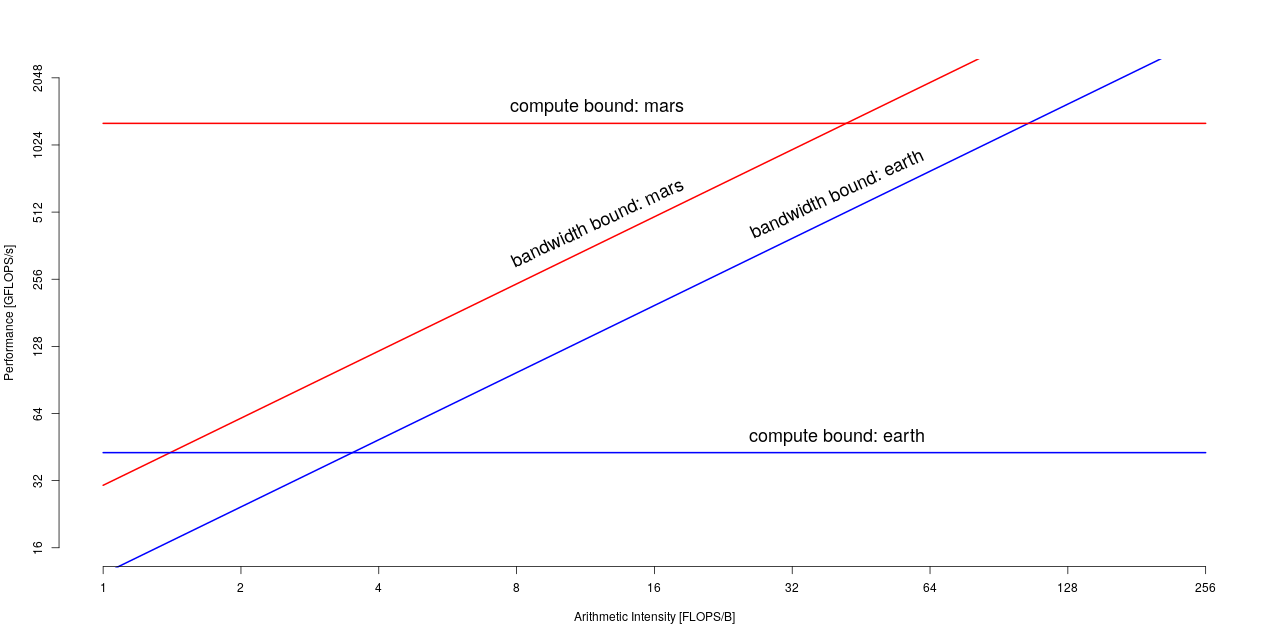
\includegraphics[scale=0.4, angle=90]{roofline-earth-mars-pure.png}


\subsection{Machine 2 / Mars}

The mars system has:
 \begin{itemize}
 	\item 8 Sockets with
	\item an Intel Xeon E7-8850 @ 2.00 GHz
	\item with 10 Cores each.
\end{itemize}

As such it is an 80 core NUMA shared memory system.

\subsubsection{Theoretical Peak Performance}

The Xeon E7-8850 is a Westermere-EX architecture based on Nehalem.\cite{wikichip}
As such is has two discrete ALU's for addition and multiplication.
Each ALU can process up to 4 SP Floats per cycle when using the appropriate SIMD instructions.\cite{agnerorg}

This results in a peak performance for the whole mars system of:
$$\text{Throughput} = 4 \text{SPF} * 2 \text{(ALUs)} * 2 Ghz * 80 = 1280 \, GFLOPs$$

\subsubsection{STREAM or NUMA-STREAM}

We measured the maximal bandwith using the NUMA-STREAM benchmark.
The maximum Bandwith measured was 30.5GB/s

\begin{center}
\begin{tabular}{|r|r|}
	\hline
	Function & MB/s    \\ \hline
	Copy     & $30344$ \\ \hline
	Scale    & $\pmb{30521}$ \\ \hline
	Add      & $30126$ \\ \hline
	Triad    & $30260$ \\ \hline
\end{tabular}
\end{center}

\subsubsection{Roofline Plot}

\begin{figure}[]
	\centering
	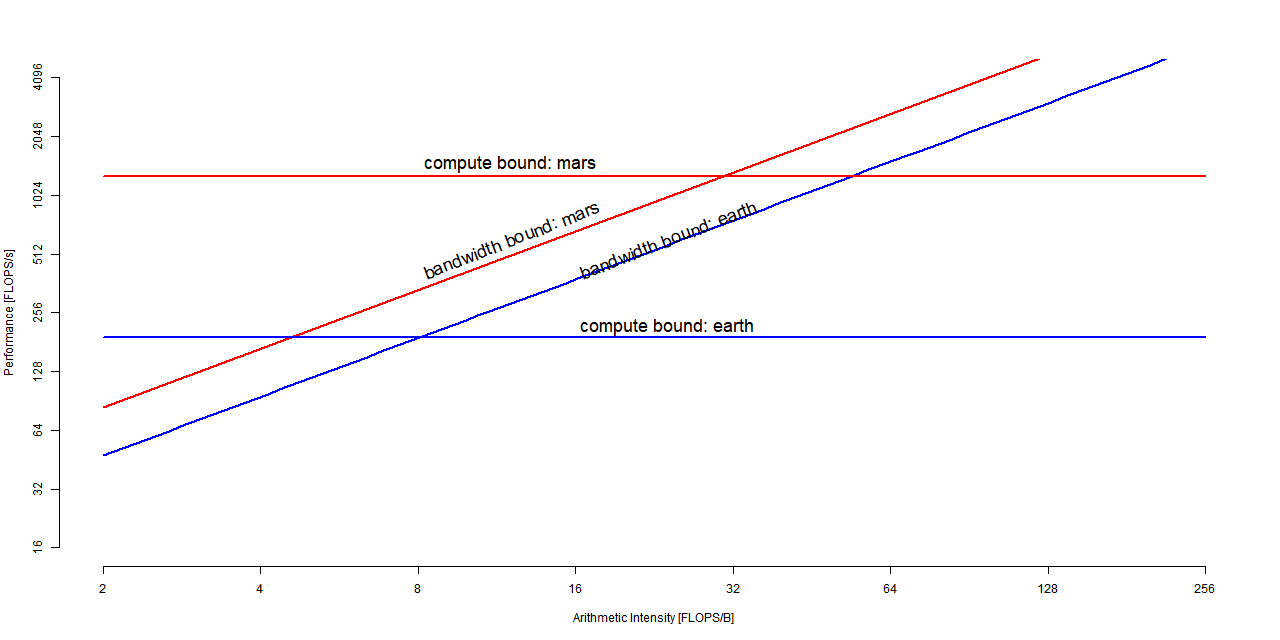
\includegraphics[width=.5\linewidth]{figures/placeholder}
	\caption{Calculated roofline model for mars}
	\label{fig:runtime}
\end{figure}

\newpage
\subsubsection{Compilation Details \& Output}

\begin{center}
\begin{lstlisting}[basicstyle=\tiny]
gcc -O3 -std=c99 stream.c -lnuma -fopenmp -DN=80000000 -DNTIMES=100 -o stream-gcc
.\stream-gcc
-------------------------------------------------------------
STREAM version $Revision: 5.9 $
-------------------------------------------------------------
This system uses 8 bytes per DOUBLE PRECISION word.
-------------------------------------------------------------
Array size = 80000000
Total memory required = 1831.1 MB.
Each test is run 100 times, but only
the *best* time for each is used.
-------------------------------------------------------------
Number of Threads requested = 80
Number of available nodes = 8
-------------------------------------------------------------
Your clock granularity/precision appears to be 1 microseconds.
Each test below will take on the order of 20711 microseconds.
(= 20711 clock ticks)
Increase the size of the arrays if this shows that
you are not getting at least 20 clock ticks per test.
-------------------------------------------------------------
WARNING -- The above is only a rough guideline.
For best results, please be sure you know the
precision of your system timer.
-------------------------------------------------------------
Function      Rate (MB/s)   Avg time     Min time     Max time
Copy:       30344.0333       0.0429       0.0422       0.0441
Scale:      30521.8913       0.0424       0.0419       0.0440
Add:        30126.6472       0.0645       0.0637       0.0656
Triad:      30260.5691       0.0643       0.0634       0.0660
-------------------------------------------------------------
Solution Validates
-------------------------------------------------------------
\end{lstlisting}
\end{center}

\section{Performance of kmeans Kernel}

\subsection{Compilation Details}

The kmeans benchmark was compiled with the following flags apply to the executable and all c files:

\begin{verbatim}
CC_FLAGS= -DLIKWID_PERFMON -g -I/opt/likwid/include -L/opt/likwid/lib -llikwid -fopenmp -O2
\end{verbatim}

\noindent GCC 7.3 was used as compiler:

\begin{verbatim}
e01426266@mars:~/NUMA-STREAM$ gcc -v
Using built-in specs.
COLLECT_GCC=gcc
COLLECT_LTO_WRAPPER=/usr/lib/gcc/x86_64-linux-gnu/7/lto-wrapper
OFFLOAD_TARGET_NAMES=nvptx-none
OFFLOAD_TARGET_DEFAULT=1
Target: x86_64-linux-gnu
Configured with: .... <omitted for breviety>
Thread model: posix
gcc version 7.3.0 (Debian 7.3.0-5)
\end{verbatim}

\noindent For performance measurements \texttt{likwid-4.3.1} was used.

\subsection{Obtain AI for kmeans}

We measured the AI of kmeans using likwid. The following schema was used for all invocations.
\begin{verbatim}
/opt/likwid/bin/likwid-perfctr -f -C <0-79/60-69> -g \
    FLOPS_SP ./kmeans_openmp/kmeans -n <threads> -i <datafile>
/opt/likwid/bin/likwid-perfctr -f -C <0-79/60-69> -g \
    MEM      ./kmeans_openmp/kmeans -n <threads> -i <datafile>
\end{verbatim}



\begin{table}[h]
\centering
\caption{\label{tab:ai_tab}Overview of AIs obtained for kmeans on Mars}
\begin{small}
\begin{tabular}{lllll}
\toprule
\#cores & file & Total GFLOPS & Total GBytes & AI (FLOPS/Byte) \\
\midrule
10 & 100 & 1.33 & 73.44 & 0.02 \\
10 & 204800.txt & 1517.92 & 476.26 & 3.19 \\
10 & 819200.txt & 2225.72 & 734.17 & 3.03 \\
10 & kdd\_cup & 3427.63 & 1061.99 & 3.23 \\
80 & 100 & 0.58 & 78.48 & 0.01 \\
80 & 204800.txt & 731.82 & 981.66 & 0.75 \\
80 & 819200.txt & 1164.44 & 1244.34 & 0.94 \\
80 & kdd\_cup & 1519.86 & 1420.36 & 1.07 \\
\bottomrule
\end{tabular}
\end{small}
\end{table}

\subsection{Roofline plots for entire kmeans application}

\begin{figure}[ht]
	\centering
	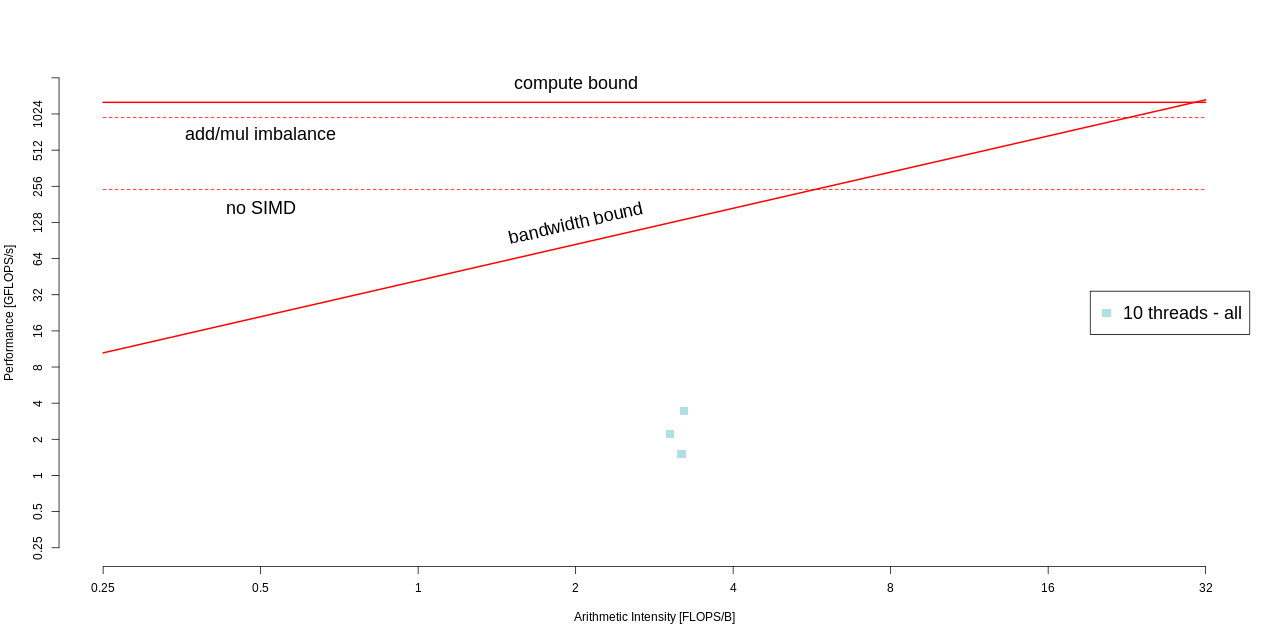
\includegraphics[width=.5\linewidth]{figures/runtime/roofline-mars-10tall.png}
	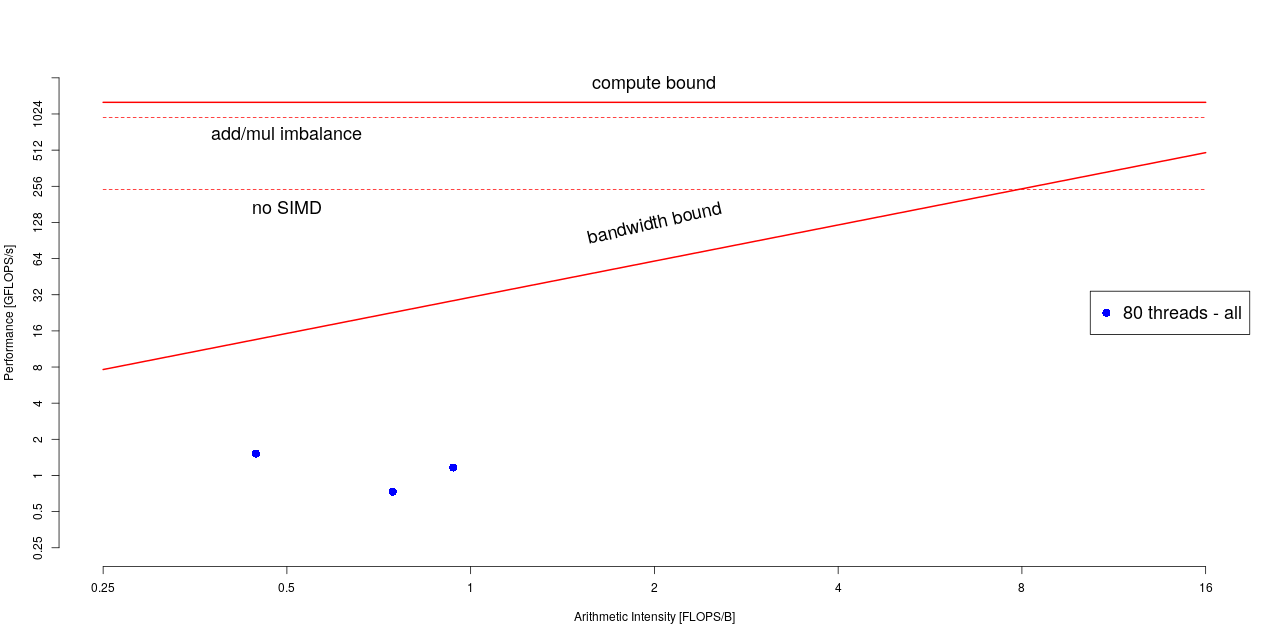
\includegraphics[width=.5\linewidth]{figures/runtime/roofline-mars-80tall.png}
	\caption{Roofline for complete kmeans application}
	\label{fig:runtime}
\end{figure}

\subsection{Roofline plots with realistic ceiling for kmeans kernel}

We arrive at a realistic Ceiling as follows:

Start with the theoretical peak performance: 1280 GFlops

Take into account the lack of SIMD parallelism:
$$\frac{1280 GFlops}{4} = 320 GFlops$$

Take into account the imbalance of MUL vs ADD operations:
$$\frac{320 GFlops}{2 Flop/Cycle} *1.5 Flop/Cycle = 240 GFlops$$

\subsection{Obtain AI for kmeans with the LIKWID marker API}

We add the -m switch to our invocations to activate the marker API.
We marked the kernel of the main loop for performance measurement.
This being the inner loop which iterates over all points of the dataset:

\begin{table}[h]
\centering
\caption{\label{tab:ai_tab}Overview of AIs obtained for kmeans on Mars}
\begin{small}
\begin{tabular}{lllll}
\toprule
\#cores & file & Total GFLOPS & Total GBytes & AI (FLOPS/Byte) \\
\midrule
10 & 100 & 385.08 & 150.01 & 2.57 \\
10 & 204800.txt & 12738.94 & 2248.92 & 5.66 \\
10 & 819200.txt & 12814.52 & 3500.45 & 3.66 \\
10 & kdd\_cup & 12995.59 & 3451.19 & 3.77 \\
80 & 100 & 7.46 & 1292.02 & 0.01 \\
80 & 204800.txt & 4017.84 & 2807.56 & 1.43 \\
80 & 819200.txt & 6579.41 & 3312.47 & 1.99 \\
80 & kdd\_cup & 5940.10 & 3230.91 & 1.84 \\

\bottomrule
\end{tabular}
\end{small}
\end{table}

\subsection{Roofline plots with realistic ceiling for kmeans kernel only (with marker API)}

\begin{figure}[ht]
	\centering
	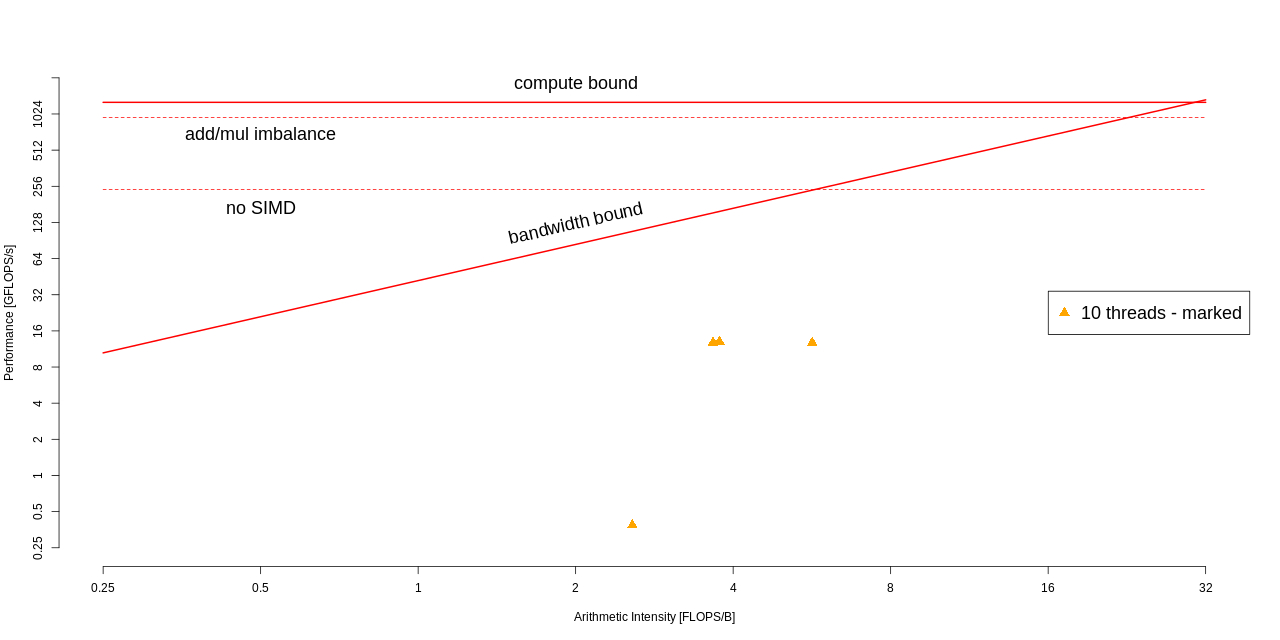
\includegraphics[width=.5\linewidth]{figures/runtime/roofline-mars-10tmarked.png}
	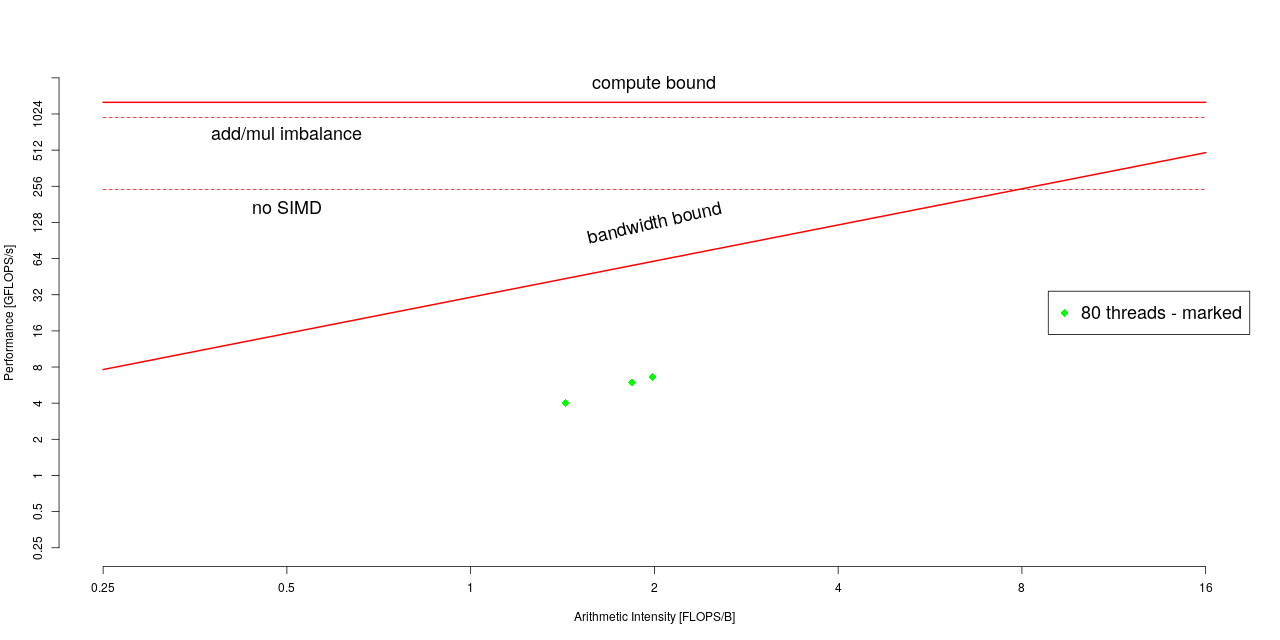
\includegraphics[width=.5\linewidth]{figures/runtime/roofline-mars-80tmarked.png}
	\caption{Roofline including realistic ceilings for Mars}
	\label{fig:runtimex}
\end{figure}


\subsection{Comparison and Discussion}

\subsubsection{Empirical AI Data}

Table \ref{tab:ai_tab} shows the recorded performance for kmeans on varius inputs.
Table \ref{tab:ai_tab_marked} improved on this data by only recording data for the kernel of the application.

When recording performance for the whole application we end up also recording parts of the program not relevant to roofline.
So we record for example during IO (reading of the input file) and initialization (allocating buffers).

As these tasks involve syscalls and possibly external hardware the are not suitable for analysis through the roofline model.
We can improve on this by only recording information about the application kernel as presented in the second table.

We can improve on our analysis even further by taking into consideration
maximum performance for the given code as discussed in \autoref{lbl:maxPerf}.

The maximum performance recorded for the marked region in a benchmark is 13GFLOPS.
According to the roofline model this would require bandwith close to $$13 GFLOPS * 0,31 Flop/Byte = 4,03 GB/s$$
However actual bandwith used for the benchmark is at $3,45 GB/s$.

So the performance of our kernel seems limited by FP performance. But we are well below the ceiling there as well.

This is likely due to reasons outside of FP performance
like branch mispredics, control flow overhead, synchronisation overhead or others. Given that performance actually goes
down when using 80 Threads compared to 10 it is an reasonable assumption that a lot of performance is lost in overhead
caused by parallelization.


\subsubsection{Maximum performance of the kmeans kernel}

The kernel of the \texttt{kmeans} algoirthm is in the \texttt{kmeans\_clustering} function.

The function is split into three main parts:
\begin{itemize}
	\item Initialization (happens once)
	\item In the main loop:
	\begin{itemize}
		\item Calculating membership to existing clusters for each point.
		\item Update clusters.
	\end{itemize}
\end{itemize}

We can safely ignore initialization for our performance consideration which leaves the main loop.

The main loop itself can be further split into three distinct parts.
\begin{itemize}
	\item For each point:
	\begin{itemize}
		\item Find the nearest cluster(\texttt{find\_nearest\_point}).
		\item Collect partial updates on the position of clusters.
	\end{itemize}
	\item Reduce partial information and update positions of clusters
\end{itemize}

For our analysis we assume 5 clusters and 34 features which matches
the default of kmeans and our input datasets.

The only significant contributors here in terms of computation are the loops to find the nearest cluster and updating the cluster information.
For this reason we will look only at these inner loops and not at the rest of the main loop.

\paragraph{}
\begin{lstlisting}[caption={Inlined representation of find\_nearest\_point}]
for (i=0; i<nclusters; i++) {
	float dist=0;
	for (j=0; j<nfeatures; j++)
		dist += (pt1[j]-clusters[i][j]) * (pt1[j]-clusters[i][j]);
	if (dist < min_dist) {
		min_dist = dist;
		index    = i;
	}
}
\end{lstlisting}
The kernel here is:
\texttt{dist += (pt1[j]-pt2[j]) * (pt1[j]-pt2[j])}.\newline

We get 8 byte of memory bandwith for three floating point operations.
Memory bandwith consists of 2 loads for each iteration:
\begin{itemize}
	\item Read: \texttt{pt1[j]}
	\item Read: \texttt{clusters[i][j]}
\end{itemize}
Operations are two additions and one multiplication.
\footnote{Treating subtraction as addition.}
\footnote{While there are two subtractions in the code gcc will eliminate one through common subexpression elimination.}


Immediatly obvious from the snippet above we get at least $nclusters * nfeatures$ iterations.
With one call to \texttt{find\_nearest\_point} for each point per iteration of the main loop this gives us:\\
$$iterations = n * \texttt{nclusters} * \texttt{nfeatures} = n * 170$$

Even for our smallest data sample which has 100 points this already gives us $17000$ iterations and will dominate the computational demands for any reasonably large size of n.

If we stop here our Arithmethic Intensity is 3 FP operations per 8 byte. Giving an AI of $\frac{0,375 Ops}{Byte}$
\footnote{Although in practice caches will usually hold both pt1 and the clusters after the first run of the loop body.}


\paragraph{}
Also for each point we will update the partial cluster information:
\begin{lstlisting}[caption={Updating (partial) cluster information},label=lblUpdPartClst]
for (j=0; j<nfeatures; j++)
partial_new_centers[tid][index][j] += feature[i][j];
\end{lstlisting}
We get for the number of iterations:
$$iterations = n * nfeatures = 34$$

While this is not as big an contributor as the loop finding the nearest cluster
it still contributes a noteworthy amount of computational demands.

In particular for each iteration here we have two loads (8 Byte) and one addition.
\footnote{Although it is fair to assume that partial\_new\_centers[tid][index][j] will be cached.}

Past this what is left to do is the combination of partial cluster information and calculating the new clusters.

\paragraph{} This happens in a fixed (relative to the number of points) number of iterations so no AI intensity calculation was done on this code.


\begin{lstlisting}[caption={Reduction pt1}]
/* let the main thread perform the array reduction */
for (i=0; i<nclusters; i++) {
	for (j=0; j<nthreads; j++) {
		new_centers_len[i] += partial_new_centers_len[j][i];
		partial_new_centers_len[j][i] = 0.0;
		for (k=0; k<nfeatures; k++) {
			new_centers[i][k] += partial_new_centers[j][i][k];
		partial_new_centers[j][i][k] = 0.0;
		}
	}
}
\end{lstlisting}

The amount of iterations of the above loop is static in regards to the number of items we work on.
It is given by $ iterations = clusters * threads * features$.
In our case when using all cores of the Mars system we get:
$$ iterations = 5 * 80  * 34 = 13600$$
However this is neglible for nontrivial datasets so we exclude it from the AI caluclation.

Similar we have the loop calculating the new clusters at the end of the main loop:
\begin{lstlisting}[caption={Reduction pt2}]
/* replace old cluster centers with new_centers */
for (i=0; i<nclusters; i++) {
	for (j=0; j<nfeatures; j++) {
		if (new_centers_len[i] > 0)
			clusters[i][j] = new_centers[i][j] / new_centers_len[i];
		new_centers[i][j] = 0.0;   /* set back to 0 */
	}
	new_centers_len[i] = 0;   /* set back to 0 */
}
\end{lstlisting}
With this loop having at most iterations of:
$$clusters * features = 5 * 34 = 170 = iterations$$
This loop has no significant impact on overall performance and can safely be ignored.

\subsection{kmeans: Roofline Model}

Table \ref{tab:AI} gives us the AI for the inner main loop based on it's two essential parts according to the roofline model.

It is however important to point out this does assume NO caching. In practice much of the memory pressure might be absorbed by the cache.

\begin{table}[ht]
	\centering
	\caption{Arithmethic Intensity according to the Roofline Model}
	\label{tab:AI}
	\begin{tabular}{|r|r|r|r|}
		\hline
		& Find nearest Cluster & Update cluster information & Total \\ \hline
		Iterations           & $n * 170$            & $n*34$                     & -     \\ \hline
		Memory (Byte)              & $8*170$              & $12*34$                      & 1768  \\ \hline
		Operations (Flop)          & $3*170$              & $1*34$                       & 544   \\ \hline
		Arithmetic Intensity (Flop/Byte) & 0,375                & 0,08                       & 0,31  \\ \hline
	\end{tabular}
\end{table}

\subsection{kmeans: Maximum Performance}

When considering the maximum performance of the given code there are multiple things to consider:

\begin{itemize}
	\item The kernel does not use SIMD instructions. This immediatly brings down maximum performance by a factor of 4!
	\item The kernel is not balanced. There is actually only a single relevant multiplication in the inner loop! Which can happen in parallel to the additions.
\end{itemize}

This means performance is limited by the addition ALU primarily.

In \texttt{find\_nearest\_point} we have two additions and one multiplication per result. This mean on average we will execute an addition every cycle and a multiplication every second.
So we execute 1,5 Instructions per cycle instead of the maximum of 2 in this kernel because of the mul/add imbalance.

We could additionally take into account the smaller loop \autoref{lblUpdPartClst} which is limited purely by addition.
However this would bring down flops/cycle only slightly to 1,41 so for simplicity we will use 1.5 for further analysis.

Maximum FP performance under these considerations is:
$$1280 GFlops * 0.25 \text{(no SIMD)}  * 0.75 \text{(imbalance)} = 240 GFlops$$.

Which gives us for the demand on the memory subsystem for 80 Threads:
$$\frac{240 GFlops}{0,31 Flop/Byte} = 774 GB/s$$

And 10 Threads:
$$\frac{30 GFlops}{0,31 Flop/Byte} = 96 GB/s$$

However since many of the inputs to the kernel can be cached this is not representative of the actualy demands on the memory system as our measurements show.

















%%%%%%%%%% DELETE IF NOT NEEDED %%%%%%%%%
\newpage

Here are templates how to insert a table or a figure into your report.

The run-time of our algorithm is shown in Figure~\ref{fig:runtime}.

\begin{figure}[ht]
\centering
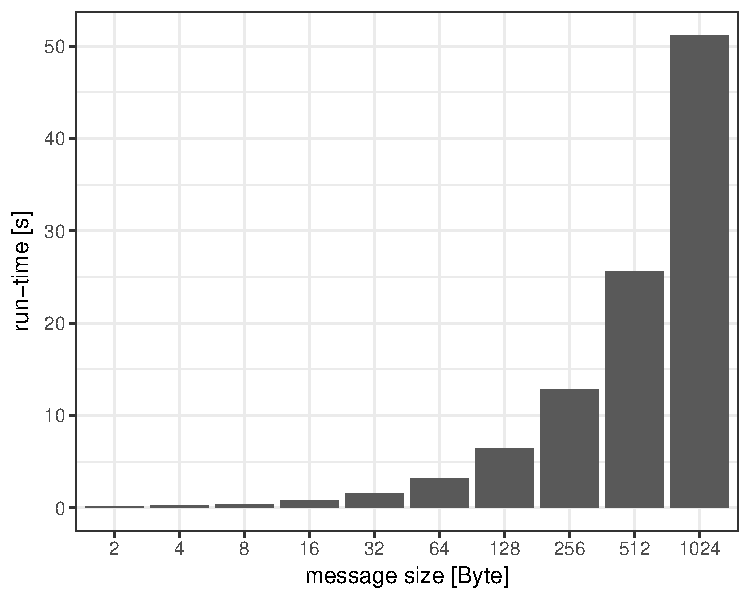
\includegraphics[width=.5\linewidth]{figures/runtime}
\caption{Run-time of algorithm X on machine Y.}
\label{fig:runtime}
\end{figure}


Table~\ref{tab:related_algorithms} shows a summary of related algorithms.

\begin{table}[ht]
\centering
\captionabove{Related algorithms and their complexity.}
\label{tab:related_algorithms}
\begin{tabular}{ll}
\toprule
algorithm & complexity \\
\midrule
algorithm Y & $O(n)$ \\
algorithm Z & $O(n \log{n} )$ \\
\bottomrule
\end{tabular}
\end{table}

We can cite a nice book of Pinedo~\cite{Pinedo:2008vs} if we want to.
